\documentclass[usepdftitle=false,hyperref={pdfpagelabels=false}]{beamer}

% use KIT-Theme
% see http://sdqweb.ipd.kit.edu/wiki/Dokumentvorlagen
%\usetheme{Frankfurt} % see http://deic.uab.es/~iblanes/beamer_gallery/index_by_theme.html as fallback
\InputIfFileExists{../templates/beamerthemekit.sty}{\usepackage{../templates/beamerthemekit}}{\usetheme{Frankfurt}}
\usefonttheme{professionalfonts}

\usepackage{hyperref}
\usepackage{lmodern}
\usepackage{listings}
\usepackage{wrapfig}        % see http://en.wikibooks.org/wiki/LaTeX/Floats,_Figures_and_Captions
\usepackage[utf8]{inputenc} % this is needed for german umlauts
\usepackage[ngerman]{babel} % this is needed for german umlauts
\usepackage[T1]{fontenc}    % this is needed for correct output of umlauts in pdf
\usepackage{verbatim}
\usepackage{relsize}
\usepackage{subfigure}
\usepackage{algorithm,algpseudocode}
\usepackage{minted}         % needed for the inclusion of source code
\usepackage{tikz}
\usetikzlibrary{shapes,snakes,calc,patterns}
\usepackage{xcolor}
\usepackage{menukeys}
\usepackage{braket}
\usepackage{ulem}
\usepackage{../templates/myStyle}

\newcommand\tutor{Martin Thoma}
\newcommand\tutNR{10}
\newcommand\titleText{Programmieren-Tutorium Nr. \tutNR{}}
\institute{Fakultät für Informatik}

\hypersetup{pdftitle={\titleText}}
\beamertemplatenavigationsymbolsempty

\newcommand\InsertToC[1][]{
  \begin{frame}{Outline}
    \tableofcontents[subsectionstyle=show/show/show, subsubsectionstyle=show/show/show, #1]
  \end{frame}
}

\begin{document}
\title{\titleText}
\subtitle{Einführung in Java, Eclipse}
\author{\tutor}
\date{\today}
\subject{Programmieren}

\frame{\titlepage}

\frame{
    \frametitle{Inhaltsverzeichnis}
    \setcounter{tocdepth}{1}
    \tableofcontents
    \setcounter{tocdepth}{2}
}

%\AtBeginSection[]{
%    \InsertToC[sections={\thesection}]  % shows only subsubsections of one subsection
%}

\section{Allgemeines}
\subsection{Formalien}
\begin{frame}{Formalien}
    \begin{itemize}
        \item Die Folien werden online gestellt $ \Rightarrow $
              \textbf{Mitschreiben nicht nötig}
        \item $\rightarrow$ \href{http://martin-thoma.com/programmieren-tutorium}{martin-thoma.com/programmieren-tutorium}
        \item Fragen immer sofort stellen – und traut euch!\\
              Wenn nicht hier, wo dann?
    \end{itemize}
\end{frame}

\subsection{Vorstellung}
\begin{frame}
    \frametitle{Das bin ich}
    \begin{itemize}
      \item Martin Thoma (\href{mailto:info@martin-thoma.de}{info@martin-thoma.de}) $\rightarrow$ \href{http://www.martin-thoma.de/about.htm}{CV}
      \item 22 Jahre alt
      \item komme aus Augsburg
      \item 3. Semester, Informatik
      \item Programmieren
        \begin{itemize}
            \item \textbf{2005}: Angefangen mit PHP (\& HTML, CSS, JavaScript, (My)SQL)
            \item \textbf{2009}: Liebe zu Python entdeckt \\
                  (\href{http://martin-thoma.com/challenge-websites/}{HackIts und Challenges} auf ProjectEuler, Brightshadows)
            \item \textbf{Selten}: C, C++ (z.B. für ein größeres Forschungsprojekt)
            \item \textbf{2011}: Java am KIT gelernt
            \item BwInf, Online-Projekte wie z.B. \href{http://world-of-dungeons.net/}{world-of-dungeons}
        \end{itemize}
    \end{itemize}
    \textbf{Und wer seid ihr?}
\end{frame}

\subsection{Websites}
\begin{frame}
    \frametitle{Websites und Links}
    \begin{itemize}
      \item \href{http://martin-thoma.com/programmieren-tutorium}{martin-thoma.com/programmieren-tutorium}:\\
            Alle Links, Folien, Hinweise und viele weitere Inhalte
      \item \href{https://praktomat.info.uni-karlsruhe.de/}{praktomat.info.uni-karlsruhe.de}:\\
            Forum; Abgabe der Übungsaufgaben; Klausur
      \item \href{https://webinscribe.ira.uka.de/}{webinscribe.de}: Anmeldung für das Tutorium
      \item \href{http://verialg.iti.kit.edu/english/583.php}{tinyurl.com/prog2012}: Website von Prof. Dr. Sinz
      \item \href{http://docs.oracle.com/javase/7/docs/}{docs.oracle.com}: Manual $\rightarrow$ \href{http://docs.oracle.com/javase/7/docs/api/}{API}
      \item \href{http://stackoverflow.com/}{stackoverflow.com}: Weitergehende Fragen
    \end{itemize}
\end{frame}

\subsection{Tutorium, Übung, Vorlesung}
\begin{frame}
    \frametitle{Tutorium, Übung, Vorlesung}
\begin{tikzpicture}[%
    auto,
    example/.style={
      rectangle,
      draw=blue,
      thick,
      fill=blue!20,
      text width=4.5em,
      align=center,
      rounded corners,
      minimum height=2em
    },
    longName/.style={
      text width=12em,
      align=center,
      minimum height=2em
    },
    algebraicName/.style={
      text width=7em,
      align=center,
      minimum height=2em
    },
    explanation/.style={
      text width=10em,
      align=left,
      minimum height=3em
    }
  ]
\pgfdeclarepatternformonly{north east lines wide}%
   {\pgfqpoint{-1pt}{-1pt}}%
   {\pgfqpoint{10pt}{10pt}}%
   {\pgfqpoint{9pt}{9pt}}%
   {
     \pgfsetlinewidth{3pt}
     \pgfpathmoveto{\pgfqpoint{0pt}{0pt}}
     \pgfpathlineto{\pgfqpoint{9.1pt}{9.1pt}}
     \pgfusepath{stroke}
    }


    % Big background
    \draw[fill=lime!20,lime!20, rounded corners]     (-1.8, 0.60) rectangle (10,-5);

    \draw[fill=purple!20,purple!20, rounded corners] (0.55, -3.1) rectangle (3.5,-3.9);
    \draw[fill=purple!20,purple!20, rounded corners] (4.55, -3.1) rectangle (7.5,-3.9);

    \draw[fill=blue!20,blue!20, rounded corners] (-1.45,-1.4) rectangle (1.5,-0.6);
    \draw[fill=blue!20,blue!20, rounded corners] (2.55,-1.4) rectangle (5.5,-0.6);
    \draw[fill=blue!20,blue!20, rounded corners] (6.55,-1.4) rectangle (9.5,-0.6);

    \draw (2, 0) node[longName] (A) {Modul: Programmieren}
          (6, 0) node[explanation]   (X) {
            \begin{minipage}{0.9\textwidth}
                \tiny
                \begin{itemize}
                    \item 5 ECTS
                \end{itemize}
            \end{minipage}
          }
          (0,-1) node[algebraicName] (B) {Tutorium}
          (4,-1) node[algebraicName] (C) {Übung}
          (8,-1) node[algebraicName] (D) {Vorlesung}
          (0,-2) node[algebraicName] (E) {Student}
          (4,-2) node[algebraicName] (F) {Mitarbeiter}
          (8,-2) node[algebraicName] (G) {Dozent}
          (2,-3.5) node[algebraicName, purple] (H) {Übungsschein}
          (1.8,-4.35) node[explanation]   (X) {
            \begin{minipage}{\textwidth}
                \tiny
                \begin{itemize} \itemsep-0.2em
                    \item Muss bestanden werden
                    \item Keine Note
                    \item keine Bonuspunkte
                \end{itemize}
            \end{minipage}
          }
          (6,-3.5) node[algebraicName, purple] (I) {Klausur}
          (5.8,-4.3) node[explanation]   (X) {
            \begin{minipage}{\textwidth}
                \tiny
                \begin{itemize} \itemsep-0.2em
                    \item Muss bestanden werden
                    \item Abschlussnote ergibt Modulnote
                \end{itemize}
            \end{minipage}
          };

    \draw[blue, thick, rounded corners] ($(B.north west)$) rectangle ($(B.south east)$);
    \draw[blue, thick, rounded corners] ($(C.north west)$) rectangle ($(C.south east)$);
    \draw[blue, thick, rounded corners] ($(D.north west)$) rectangle ($(D.south east)$);

    \draw[purple, thick, rounded corners] ($(H.north west)$) rectangle ($(H.south east)$);
    \draw[purple, thick, rounded corners] ($(I.north west)$) rectangle ($(I.south east)$);

    \draw[lime, thick, rounded corners]   ($(B.north west)+(-0.1,0.1)$) rectangle ($(E.south east)+(0.1,-0.1)$);
    \draw[lime, thick, rounded corners]   ($(C.north west)+(-0.1,0.1)$) rectangle ($(F.south east)+(0.1,-0.1)$);
    \draw[lime, thick, rounded corners]   ($(D.north west)+(-0.1,0.1)$) rectangle ($(G.south east)+(0.1,-0.1)$);
\end{tikzpicture}
\end{frame}

\subsection{Was ist der Job eines Tutors?}
\begin{frame}
    \frametitle{Was ist der Job eines Tutors?}
    \begin{itemize}
      \item Fragen zum Stoff beantworten
        \begin{itemize}
          \item Gerne auch \emph{etwas} darüber hinaus
        \end{itemize}
      \item Fragen zur Vorlesung beantworten
        \begin{itemize}
          \item z.B. Klausurmodalitäten
        \end{itemize}
      \item Übungsblätter korrigieren
    \end{itemize}
\end{frame}

\subsection{Was ist nicht der Job eines Tutors?}
\begin{frame}
    \frametitle{Was ist \underline{nicht} der Job eines Tutors?}
    \begin{itemize}
      \item Vorlesung wiederholen
      \item Bespaßung im Tutorium
      \item Jeden durch die Klausur bringen
      \item \dots oder die Korrektur der Klausur
    \end{itemize}
\end{frame}

\subsection{Für was ist der Student verantwortlich?}
\begin{frame}
    \frametitle{Für was ist der Student verantwortlich?}
    Der Student ist für sich selbst verantwortlich, also \dots
    \begin{itemize}
      \item \dots die rechtzeitige Übungsblattabgabe
      \item \dots die Vor- und Nachbereitung der Vorlesung
      \item \dots das Lernen der Inhalte
      \item \dots die rechtzeitige Klausuranmeldung
      \item \dots das Finden relevanter Informationen
    \end{itemize}
\end{frame}

\subsection{Warnung!}

\subsection{Erinnerungen}
\begin{frame}{Erinnerungen}

\begin{block}{Praktomat-Anmeldung}
\url{https://praktomat.info.uni-karlsruhe.de/praktomat\_2012\_WS/}
\begin{itemize}
\item Deadline: \textbf{Freitag, 02. November 2012}
\end{itemize}
\end{block}

\begin{block}{Disclaimer: \href{http://tinyurl.com/prog-disclaimer}{tinyurl.com/prog-disclaimer}}
\begin{itemize}
\item PDF im VAB
\item Abgabe in den Briefkasten der Vorlesung Programmieren\\(Gebäude 50.34, Keller)
\item Deadline: \textbf{Freitag, 02. November 2012}
\end{itemize}
\end{block}

\begin{block}{Übungsschein \href{studium.kit.edu}{http://studium.kit.edu}}
\begin{itemize}
\item Anmeldung für den Übungsschein
\item Deadline: \textbf{Sonntag, 31. März 2013}
\end{itemize}
\end{block}
\end{frame}

\subsection{Nicht abschreiben!}
\begin{frame}{Nicht abschreiben!}
\begin{alertblock}{Warnung!}
\begin{itemize}
\item \emph{\textbf{Nicht abschreiben!}}
\item Schon bei \textbf{einmaligem} Nachweis verwirkt man die Chance auf den \textbf{Übungsschein}
\item Ohne Schein darf man die \textbf{Abschlussaufgabe} nicht schreiben
\item Nur mit beidem besteht man das \textbf{Modul Programmieren}
\item Programmieren ist Teil der \textbf{Orientierungsprüfung}
\item Ohne bestandene Orientierungsprüfung bis zum 3. Semester \textbf{fällt man aus dem Studium} und darf bundesweit das Studienfach nicht mehr belegen!
\end{itemize}
\end{alertblock}
\end{frame}

\subsection{Praktomat}
\begin{frame}{Praktomat}
    \begin{itemize}
        \item Ihr könnt beliebig häufig Lösungen hochladen!
        \item Ladet Teillösungen hoch
        \begin{itemize}
            \item[$\Rightarrow$] Sicherungskopie für euch
            \item[$\Rightarrow$] Eine vergessene Deadline ist nicht ganz so ärgerlich
        \end{itemize}
        \item Rechnet nicht mit der Erreichbarkeit des Praktomaten
              kurz vor der Deadline
        \item \textbf{Disclaimer nicht vergessen!}
    \end{itemize}
\end{frame}

\section{Was ist Programmieren?}
\subsection{Algorithmen}
\begin{frame}
    \frametitle{Algorithmen}
    \begin{block}{Allgemeines}
      \begin{itemize}
        \item Modul des 2. Semesters
        \item 6 ECTS
      \end{itemize}
    \end{block}
    \begin{block}{Themen}
      \begin{itemize}
        \item Sortieralgorithmen
        \item Suchalgorithmen
        \item Speicherplatz- und Laufzeitkomplexität
        \item Weiterführende Datenstrukturen (Stack, Heap, B-Bäume, \dots)
      \end{itemize}
    \end{block}
\end{frame}

\subsection{SWT - Softwaretechnik}
\begin{frame}
    \frametitle{SWT - Softwaretechnik}
    oder auch "`Programmieren im Großen"'
    \begin{block}{Allgemeines}
      \begin{itemize}
        \item Modul des 2. Semesters
        \item 6 ECTS
      \end{itemize}
    \end{block}
    \begin{block}{Themen}
      \begin{itemize}
        \item Wie gehe ich die Entwicklung von Software an?
        \item Wie strukturiere ich Programme?
        \item Wie entwickle ich \emph{leicht} wartbare Software?
        \item Entwurfsmuster
        \item Wasserfallmodell, Scrum, V-Modell
      \end{itemize}
    \end{block}
\end{frame}

\subsection{Programmieren}
\begin{frame}
    \frametitle{Programmieren}
    oder auch "`Programmieren im Kleinen"'
    \begin{block}{Allgemeines}
      \begin{itemize}
        \item Modul des 1. Semesters
        \item 5 ECTS
        \item Teil der Orientierungsprüfung
      \end{itemize}
    \end{block}
    \begin{block}{Themen}
      \begin{itemize}
        \item \textbf{Allgemeines}: Was ist eine if-Abfrage, was eine for- bzw. while-Schleife?
        \item Wie mache ich meinen Code wartbar?
        \item \textbf{Objektorientierung}: Was ist eine Klasse, was ein Objekt?
        \item Modellierung von Problemen
        \item \textbf{Elementare Datenstrukturen und -typen}: int, String, Array
      \end{itemize}
    \end{block}
\end{frame}

\section{Java}
\subsection{Begriffe}
\begin{frame}{Begriffe}
    \begin{block}{JDK}
        Das Java Development Kit (JDK) ist eines der von
        Java-Entwicklern meistgenutzten Java-SDKs.\\
        $[\dots]$ Nun wird eine angepasste freie Version als ihr nunmehr
        offizieller Nachfolger unter dem Namen OpenJDK weitergeführt.
    \end{block}

    \begin{block}{JRE}
        Die Java-Laufzeitumgebung (englisch: Java Runtime Environment, kurz JRE)
        ist die Laufzeitumgebung der Java-Technik. Mit ihr werden
        Programme (Java-Anwendungen) weitgehend unabhängig vom
        darunter liegenden Betriebssystem ausgeführt.
    \end{block}

    Quelle: Wikipedia
\end{frame}

\subsection{Workflow}
\framedgraphic{Workflow}{schaubild-java-workflow.png}

\section{System einrichten}
\subsection{Linux}
\begin{frame}{Java unter Linux}
    \begin{itemize}
        \item Ubuntu: \href{http://wiki.ubuntuusers.de/Java/Installation}{UbuntuUsers.de}\\
              \myCode{\$ sudo apt-get install openjdk-7-jre openjdk-7-jdk}
        \item Arch: \href{https://wiki.archlinux.de/title/Java}{archlinux.de}\\
              \myCode{\$ pacman -S jre7-openjdk}
    \end{itemize}
\end{frame}

\subsection{Windows}
\begin{frame}{Windows}
    \begin{itemize}
        \item \href{http://java.com/de/download/index.jsp}{java.com/download}
    \end{itemize}
    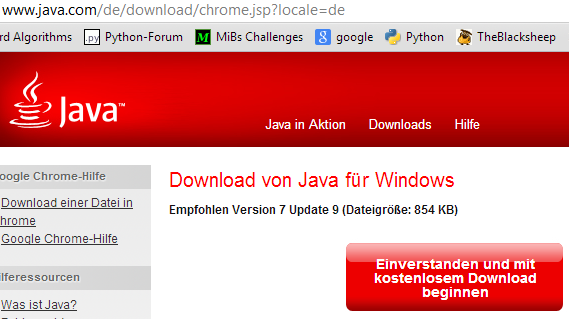
\includegraphics[width=100mm]{java-download.png}
\end{frame}

\begin{frame}{Windows - 32 oder 64 Bit Version?}
    \menu{Start > Systemsteuerung} oder \keys{Windows + Pause}
    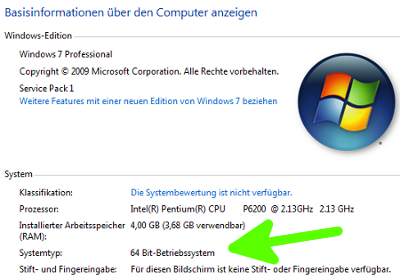
\includegraphics{windows-systemsteuerung.png}
\end{frame}

\begin{frame}{Windows - cmd}
    \begin{itemize}
        \item Ausführen: \myCode{cmd}
        \item \myCode{> javac -version}
        \item \myCode{javac 1.7.0\_09} $\rightarrow$ hat geklappt
        \item Sonst: javac zu PATH hinzufügen
            \begin{enumerate}
                \item Wo liegt "`javac.exe"'?\\(z.B. \directory{C:/Program Files/Java/jdk1.7.0\_09/bin/javac.exe})
                \item Systemsteuerung (\keys{Windows + Pause})\\
                      \menu{Systemsteuerung > Erweiterte Systemeinstellungen > Umgebungsvariablen}
                \item Zu "`Path"' durch \myCode{;} getrennt hinzufügen
            \end{enumerate}
    \end{itemize}
\end{frame}

\subsection{Java testen}
\begin{frame}{Java testen}
    \inputminted[linenos, numbersep=5pt, tabsize=4, frame=lines, label=HelloWorld.java]{java}{HelloWorld.java}
    \inputminted[linenos=false]{console}{Bash.sh}
\end{frame}

\subsection{Eclipse: Allgemeines}
\begin{frame}{Eclipse: Allgemeines}
    \begin{itemize}
        \item Sehr komfortable Java-IDE:
        \begin{itemize}
            \item Syntaxhighlighting und Code-Vervollständigung
            \item Automatisch korrektes Einrücken mit \keys{\ctrl + \shift + F})
        \end{itemize}
        \item Sehr groß (RAM \& HDD)
        \item Startet Langsam
        \item Müsst ihr in SWT verwenden
        \item Download: \href{http://www.eclipse.org/}{eclipse.org}
    \end{itemize}
\end{frame}

\subsection{Eclipse: Einrichten}
\begin{frame}{Eclipse: Einrichten}
    \begin{itemize}
        \item \menu{Window > Open Perspective > Java}
        \item \menu{Window > Show Toolbar}
        \item \menu{Window > Preferences > General > Editors > Text Editors}
            \begin{itemize}
                \item Show line numbers
                \item Print margin column: 120
            \end{itemize}
    \end{itemize}
\end{frame}

\framedgraphic{Zwischenstand}{eclipse-einrichten.png}

\subsection{Eclipse: Erstes Projekt}
\begin{frame}{Eclipse: Erstes Projekt}
    \begin{itemize}
        \item \menu{File > New > Java}: Projektname: HelloWorld
        \item \menu{File > New > Class}: Name: HelloWorld
    \end{itemize}
\end{frame}

\framedgraphic{Zwischenstand}{eclipse-projekt.png}

\section{Wiederholung}
\subsection{Begriffe}
\begin{frame}{Begriffe}
    Welche Begriffe habt ihr in der Vorlesung kennen gelernt?
\end{frame}

\begin{frame}{Begriffe}
    \begin{itemize}
        \item \textbf{Objekt}: Exemplar eines bestimmten Datentyps
        \item \textbf{Klasse}: abstraktes Modell für eine Reihe von ähnlichen Objekten
        \item \textbf{Variable}: Behälter für Werte
        \item \textbf{Konstante}: Wert, der sich während der Laufzeit des Programms nicht ändern kann
        \item \textbf{Attribut}: Eigenschaft eines konkreten Objekts
        \item \textbf{Funktion}: Programmkonstrukt mit Parametern und Rückgabewert
        \item \textbf{Methode}: Funktion in einem Objekt
        \item \textbf{Datentyp}: Zusammenfassung von Objektmengen mit den darauf definierten Operationen
        \item int, Integer
        \item String
        \item \dots
    \end{itemize}
\end{frame}

\subsection{Beispiel für eine Klasse}
\begin{frame}{Beispiel für eine Klasse}
    \begin{block}{Schal}
        \begin{itemize}
            \item hat eine Farbe
            \item besteht aus einem Stoff
            \item hat eine Länge
            \item kann warm halten
        \end{itemize}
    \end{block}
\end{frame}

\subsection{Java: Primitive Datentypen}
\begin{frame}{Java: Primitive Datentypen}
    \begin{tabular}{l|l|l}
        Datentyp    & Werte                                             & Länge\\
        \hline
        \hline
        boolean     & \texttt{true} oder \texttt{false}                         & 1 Byte\\
        char        & 16-Bit Unicode Zeichen                            & 2 Byte\\
        \hline
        byte        & $-2^7 =-128 \dots 2^7-1$                          & 1 Byte\\
        short       & $-2^{15}=-32\,768 \dots 2^{15}-1$                 & 2 Byte\\
        int         & $-2^{31}\approx-2 \cdot 10^9 \dots 2^{31}-1$      & 4 Byte\\
        long        & $-2^{63}=-9\cdot 10^{18} \dots 2^{63}-1$          & 8 Byte\\
        \hline
        float       & single-precision 32-bit IEEE 754 floating point   & 4 Byte\\
        double      & double-precision 64-bit IEEE 754 floating point   & 8 Byte\\
    \end{tabular}
    \\
    Quelle: \href{http://docs.oracle.com/javase/tutorial/java/nutsandbolts/datatypes.html}{docs.oracle.com}
\end{frame}

\subsection{Java: Enum}
\begin{frame}{Java: Enum}
    \inputminted[linenos, numbersep=5pt, tabsize=4, frame=lines, label=Day.java]{java}{Day.java}
    Quelle: \href{http://docs.oracle.com/javase/tutorial/java/javaOO/enum.html}{docs.oracle.com}
    \inputminted[linenos, numbersep=5pt, tabsize=4, frame=lines, label=SomeClass.java]{java}{SomeClass.java}
\end{frame}

\subsection{Java: String}
\begin{frame}{Java: String}
    \begin{itemize}
        \item \textbf{Klasse} für Zeichenketten
        \item UTF-16
        \item max. $2^{31}-1 = 2\,147\,483\,647$ Zeichen (siehe \href{http://stackoverflow.com/a/816152/562769}{stackoverflow.com})
          \begin{itemize}
            \item King James Bible: $4\,397\,206$ Zeichen\\
                  (\href{http://printkjv.ifbweb.com/\#downloads}{Quelle} \& \myCode{wc -w file.txt})
          \end{itemize}
        \item weitere Informationen: \href{http://docs.oracle.com/javase/7/docs/api/java/lang/String.html}{docs.oracle.com}
    \end{itemize}
\end{frame}

\subsection{Java: Naming Conventions}
\begin{frame}{Java: Naming Conventions}
    \begin{itemize}
        \item \myCode{camelCase} für Variablen und Attribute
        \item \myCode{BIG\_AND\_FAT} für Konstanten
        \item Typische Variablen- und Methodennamen:
          \begin{itemize}
            \item isSomething: Meist für \texttt{boolean}
            \item hasSomething: Meist Methode mit Rückgabewert \texttt{boolean}
            \item getValue: Getter, Wrapper für Attribut "`value"'
            \item setValue: Setter, Wrapper für Attribut "`value"'
          \end{itemize}
        \item Genauer: \href{http://www.oracle.com/technetwork/java/codeconventions-150003.pdf}{orcacle.com}, ab S. 15
    \end{itemize}
\end{frame}

\subsection{Aufgabenstellung}
\begin{frame}{Aufgabenstellung}
    \begin{alertblock}{Bitte achtet auf folgendes:}
        \begin{itemize}
            \item Einsatz sinnvoller Datentypen
            \item aussagekräftige Attributnamen
            \item Einrückungen, Namenskonventionen, Dokumentation
        \end{itemize}
    \end{alertblock}
\end{frame}

\section{Abspann}
\subsection{Hinweise zum Übungsblatt}
    \begin{frame}{Hinweise zum Übungsblatt}
    \begin{itemize}
        \item Aufgaben online im \textbf{Praktomaten} oder im \textbf{VAB}
        \item Abgabetermin: Montag, der \textbf{5. November 2012, 13 Uhr}
        \item Abgabe online im Praktomaten\\
              Uni-Netz oder VPN erforderlich!
        \item min. \textbf{50 \% der Gesamtpunktzahl} zum Bestehen des Scheins\\
              (ca. 60 Punkte)
        \item \textbf{keine Bibliotheken} verwenden, die im Übungsblatt nicht explizit zugelassen wurden
        \item keine ungewollte Funktionalität einbauen – es gilt die Devise:\\ \textbf{Einfache Fragen erfordern einfache Antworten!}
    \end{itemize}
\end{frame}

\subsection{Dropbox Space Race}
    \begin{frame}{Dropbox Space Race}
    \begin{itemize}
        \item Hat nichts mit Programmieren zu tun
        \item Bei \href{https://www.dropbox.com/spacerace}{dropbox.com} anmelden
        \item KIT ist auf Platz 3, RWTH Aachen und TU München vor uns
    \end{itemize}
\end{frame}

\subsection{Comic}
\framedgraphic{Vielen Dank für eure Aufmerksamkeit!}{../images/Teach-yourself-C++-in-21-days.png}

\end{document}
